\subsection{Directed and Undirected Graphical Models}

Graphical models use graph structure to encode conditional independence and to organize high-dimensional probability laws.

\begin{definition} \label{def:sl-directed-graphical-model} \hlt{Directed Graphical Model}\\
Let $G=(V,E)$ be a directed acyclic graph with $V=\{1,\ldots,d\}$ and $\operatorname{pa}(j)=\{i\in V:i\to j\in E\}$.\\
For $x=(x_1,\ldots,x_d)$, write $x_{\operatorname{pa}(j)}=(x_i)_{i\in\operatorname{pa}(j)}$. A law for $X=(X_1,\ldots,X_d)$ with joint density or mass function $p$ \hlt{factorizes according to} $G$ if $p(x)=\prod\limits_{j=1}^d p(x_j\mid x_{\operatorname{pa}(j)})$, with $p(x_j\mid x_\varnothing)\defeq p(x_j)$.
\end{definition}

\begin{definition} \label{def:sl-undirected-markov-vocabulary} \hlt{Markov Graph Vocabulary}\\
Let $G=(V,E)$ be an undirected graph, and let $A,B,C\subseteq V$ be disjoint.
\begin{enumerate}[label=(\roman*)]
\setlength{\itemsep}{0pt}
\item Vertices $j,k\in V$ are \hlt{adjacent} iff $\{j,k\}\in E$.
\item A \hlt{path} from $u$ to $v$ is $(v_0,\ldots,v_m)$ with $v_0=u$, $v_m=v$, and $\{v_{\ell-1},v_\ell\}\in E$ for $\ell=1,\ldots,m$.
\item $C$ \hlt{separates} $A$ and $B$ iff every path from $a\in A$ to $b\in B$ contains a vertex in $C$.
\item A \hlt{clique} is $K\subseteq V$ such that $\{j,k\}\in E$ for all distinct $j,k\in K$.\\
It is \hlt{maximal} iff no strictly larger clique contains $K$.
\end{enumerate}
\end{definition}

\begin{definition} \label{def:sl-markov-random-field} \hlt{Undirected Graphical Model}\\
Let $G=(V,E)$ be an undirected graph, let $\mathcal{C}$ be its maximal cliques, and let $p$ be a positive joint density or mass function for $X=(X_j)_{j\in V}$. For $C\subseteq V$, write $x_C=(x_j)_{j\in C}$. The following are equivalent:
\begin{enumerate}[label=(\roman*)]
\setlength{\itemsep}{0pt}
\item $p$ is \hlt{Markov with respect to} $G$: if $j\neq k$ and $\{j,k\}\notin E$, then $X_j\perp\!\!\!\perp X_k\mid X_{V\setminus\{j,k\}}$.
\item $p$ factorizes as $p(x)=Z^{-1}\prod\limits_{C\in\mathcal{C}}\psi_C(x_C)$ for clique potentials $\psi_C\geq0$, with $Z=\sum_x\prod\limits_{C\in\mathcal{C}}\psi_C(x_C)$ in the discrete case and $Z=\int\prod\limits_{C\in\mathcal{C}}\psi_C(x_C)\,dx$ in the continuous case.
\end{enumerate}
\end{definition}

\begin{proposition} \label{prop:sl-gaussian-graphical-precision-zeros} \hlt{Gaussian Graphical Zeros}\\
Let $X\sim N_d(\mu,\Sigma)$ with $\Sigma\succ0$ and $\Theta=\Sigma^{-1}=(\theta_{jk})$. For $j$, write $\theta_{-j,j}=(\theta_{\ell j})_{\ell\neq j}$ and $\mu_{-j}=(\mu_\ell)_{\ell\neq j}$. Then:
\begin{enumerate}[label=(\roman*)]
\setlength{\itemsep}{0pt}
\item For $z\in\mathbb{R}^{d-1}$, $\mathbb{E}[X_j\mid X_{-j}=z]=\mu_j-\frac{\theta_{-j,j}^T(z-\mu_{-j})}{\theta_{jj}}$.
\item For $j\neq k$, $X_j\perp\!\!\!\perp X_k\mid X_{-(j,k)}$ iff $\theta_{jk}=0$.
\end{enumerate}
\begin{proof}
\begin{enumerate}[label=(\roman*)]
\setlength{\itemsep}{0pt}
\item Let $Y=X_j$ and $Z=X_{-j}$. Order coordinates as $(Z,Y)$, with covariance block $\Sigma_{ZZ}$, cross-covariance $\sigma_{Zj}$.\\
Gaussian conditioning gives $\mathbb{E}[Y\mid Z=z]=\mu_j+(z-\mu_{-j})^T\Sigma_{ZZ}^{-1}\sigma_{Zj}$.\\
From $\Sigma\Theta=I$, the $(Z,j)$ block gives $\Sigma_{ZZ}\theta_{-j,j}+\sigma_{Zj}\theta_{jj}=0$, hence $\Sigma_{ZZ}^{-1}\sigma_{Zj}=-\frac{\theta_{-j,j}}{\theta_{jj}}$.
\item Let $A=\{j,k\}$ and $B=A^c$. The conditional Gaussian law of $X_A\mid X_B$ has precision $\Theta_{AA}=\left(\begin{smallmatrix}\theta_{jj}&\theta_{jk}\\ \theta_{jk}&\theta_{kk}\end{smallmatrix}\right)$. A bivariate Gaussian has independent coordinates iff its precision is diagonal, so $X_j\perp\!\!\!\perp X_k\mid X_B$ iff $\theta_{jk}=0$.
\end{enumerate}
\hlt{Structural Commentary}: Conditioning turns precision entries into regression interactions.\\
\hlt{Key Insight}: Gaussian conditional independence is zero conditional precision.
\end{proof}
\end{proposition}

\begin{definition} \label{def:sl-ising-model} \hlt{Ising Model}\\
Let $E\subseteq\{\{j,k\}:1\leq j<k\leq p\}$, set $x_0=1$, $\widetilde E=E\cup\{\{0,j\}:1\leq j\leq p\}$, and $\mathcal{N}(j)=\{k:\{j,k\}\in E\}$.\\
A \hlt{pairwise Ising model} for $X\in\{0,1\}^p$ is specified by:
\begin{enumerate}[label=(\roman*)]
\setlength{\itemsep}{0pt}
\item Joint law $p_\Theta(x)=\exp\left\{\sum\limits_{\{j,k\}\in\widetilde E}\theta_{jk}x_jx_k-\Phi(\Theta)\right\}$, where $\Phi(\Theta)=\log\sum\limits_{x\in\{0,1\}^p}\exp\left\{\sum\limits_{\{j,k\}\in\widetilde E}\theta_{jk}x_jx_k\right\}$.
\item Node conditionals $\mathbb{P}_\Theta(X_j=1\mid X_{-j}=x_{-j})=\left(1+\exp\left\{-\theta_{0j}-\sum\limits_{k\in\mathcal{N}(j)}\theta_{jk}x_k\right\}\right)^{-1}$ for $j=1,\ldots,p$.
\end{enumerate}
For $\{j,k\}\in E$, $\theta_{jk}$ is the conditional log-odds interaction between nodes $j$ and $k$.
\end{definition}

\begin{definition} \label{def:sl-restricted-boltzmann-machine} \hlt{Restricted Boltzmann Machine}\\
Let $v\in\{0,1\}^p$ be visible units, let $h\in\{0,1\}^q$ be hidden units, and let $\sigma(t)=(1+\exp(-t))^{-1}$.\\
A \hlt{restricted Boltzmann machine} is specified by:
\begin{enumerate}[label=(\roman*)]
\setlength{\itemsep}{0pt}
\item Graph restriction: no visible-visible or hidden-hidden edges.
\item Joint law $p(v,h)=Z^{-1}\exp(a^Tv+b^Th+v^TWh)$ with $a\in\mathbb{R}^p$, $b\in\mathbb{R}^q$, and $W\in\mathbb{R}^{p\times q}$.
\item Conditional factorization: $p(v\mid h)=\prod\limits_{j=1}^p\operatorname{Bern}(v_j;\sigma(a_j+W_{j\cdot}h))$ and $p(h\mid v)=\prod\limits_{k=1}^q\operatorname{Bern}(h_k;\sigma(b_k+W_{\cdot k}^Tv))$.
\end{enumerate}
In supervised variants, $v$ may concatenate feature and label units.
\end{definition}

\begin{figure}[H]
\centering
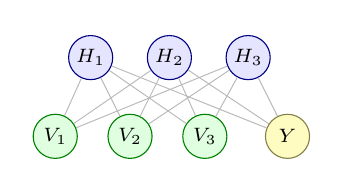
\begin{tikzpicture}[
  every node/.style={font=\scriptsize},
  unit/.style={circle, draw=gray!65, minimum size=0.56cm, inner sep=0pt},
  visible/.style={unit, fill=green!12, draw=green!50!black},
  labelunit/.style={unit, fill=yellow!24, draw=yellow!45!black},
  hidden/.style={unit, fill=blue!10, draw=blue!50!black},
  edge/.style={gray!55, line width=0.35pt}
]
  \path[use as bounding box] (-0.35,-0.38) rectangle (3.35,1.38);

  \node[visible] (v1) at (0.00,0) {$V_1$};
  \node[visible] (v2) at (0.95,0) {$V_2$};
  \node[visible] (v3) at (1.90,0) {$V_3$};
  \node[labelunit] (y) at (2.95,0) {$Y$};

  \node[hidden] (h1) at (0.45,1.00) {$H_1$};
  \node[hidden] (h2) at (1.45,1.00) {$H_2$};
  \node[hidden] (h3) at (2.45,1.00) {$H_3$};

  \foreach \v in {v1,v2,v3,y}
    \foreach \h in {h1,h2,h3}
      \draw[edge] (\v) -- (\h);
\end{tikzpicture}

\caption{RBM: \textcolor{blue!50!black}{$H_j$} connect only to visible features \textcolor{green!50!black}{$V_i$} and label \textcolor{yellow!45!black}{$Y$}; no within-layer edges.}
\label{fig:sl-restricted-boltzmann-machine-layers}
\end{figure}

\begin{remark} \label{rem:sl-separation-graphical-models} \hlt{Separation}\\
For disjoint vertex sets $A,B,C$, separation is a graphical certificate for $X_A\perp\!\!\!\perp X_B\mid X_C$: DAGs use d-separation, while undirected graphs use path separation by $C$.\\
In a Markov graph, $C$ separates $A$ and $B$ implies $X_A\perp\!\!\!\perp X_B\mid X_C$.\\
Missing edges give pairwise certificates; separation gives setwise certificates.
\end{remark}
